

\tikzset{every picture/.style={line width=0.75pt}} %set default line width to 0.75pt        

\begin{tikzpicture}[x=0.75pt,y=0.75pt,yscale=-1,xscale=1]
%uncomment if require: \path (0,300); %set diagram left start at 0, and has height of 300

%Image [id:dp32150908690987645] 
\draw (327,150) node  {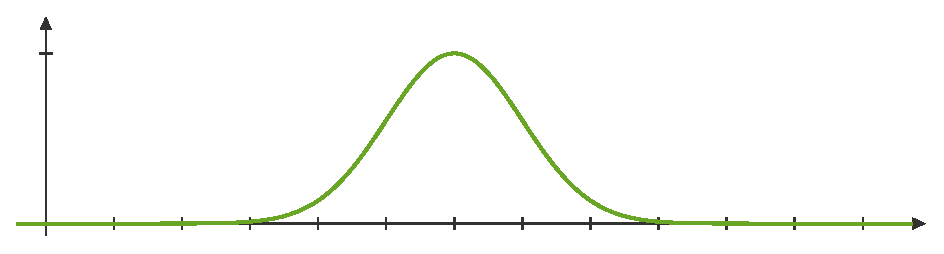
\includegraphics[width=439.5pt,height=105pt]{images/image_energy_gauss}};
%Straight Lines [id:da07666169968429992] 
\draw [color={rgb, 255:red, 155; green, 155; blue, 155 }  ,draw opacity=1 ] [dash pattern={on 4.5pt off 4.5pt}]  (63,103.4) -- (306,103.4) ;
%Straight Lines [id:da12384412498194441] 
\draw [color={rgb, 255:red, 155; green, 155; blue, 155 }  ,draw opacity=1 ] [dash pattern={on 4.5pt off 4.5pt}]  (315.6,201) -- (315.6,103) ;
%Shape: Circle [id:dp581375357919033] 
\draw  [fill={rgb, 255:red, 255; green, 255; blue, 255 }  ,fill opacity=1 ] (313.6,103.5) .. controls (313.6,102.4) and (314.5,101.5) .. (315.6,101.5) .. controls (316.7,101.5) and (317.6,102.4) .. (317.6,103.5) .. controls (317.6,104.6) and (316.7,105.5) .. (315.6,105.5) .. controls (314.5,105.5) and (313.6,104.6) .. (313.6,103.5) -- cycle ;

% Text Node
\draw (626,205.4) node [anchor=north west][inner sep=0.75pt]  [font=\footnotesize]  {$t_{\mathrm{S}}$};
% Text Node
\draw (34,59.4) node [anchor=north west][inner sep=0.75pt]  [font=\footnotesize]  {$\Phi _{\mathrm{G}}( t_{\mathrm{S}})$};
% Text Node
\draw (15,97.4) node [anchor=north west][inner sep=0.75pt]  [font=\footnotesize]  {$\Phi _{\mathrm{max}}$};
% Text Node
\draw (143,220.4) node [anchor=north west][inner sep=0.75pt]  [font=\footnotesize]  {$t_{\mathrm{S,r}} =t_{0} -3\tau _{\mathrm{S}}$};
% Text Node
\draw (162,240) node [anchor=north west][inner sep=0.75pt]  [font=\footnotesize] [align=left] {Sunrise};
% Text Node
\draw (298,240) node [anchor=north west][inner sep=0.75pt]  [font=\footnotesize] [align=left] {Noon};
% Text Node
\draw (287.5,220.4) node [anchor=north west][inner sep=0.75pt]  [font=\footnotesize]  {$t_{0} =12\mathrm{h}$};
% Text Node
\draw (403.1,220.4) node [anchor=north west][inner sep=0.75pt]  [font=\footnotesize]  {$t_{\mathrm{S,s}} =t_{0} +3\tau _{\mathrm{S}}$};
% Text Node
\draw (424,240) node [anchor=north west][inner sep=0.75pt]  [font=\footnotesize] [align=left] {Sunset};
% Text Node
\draw (564,220.4) node [anchor=north west][inner sep=0.75pt]  [font=\footnotesize]  {$2t_{0}$};
% Text Node
\draw (551,240) node [anchor=north west][inner sep=0.75pt]  [font=\footnotesize] [align=left] {Midnight};
% Text Node
\draw (44,220.4) node [anchor=north west][inner sep=0.75pt]  [font=\footnotesize]  {$0\mathrm{h}$};
% Text Node
\draw (14,240) node [anchor=north west][inner sep=0.75pt]  [font=\footnotesize] [align=left] {New solar day};


\end{tikzpicture}


